\documentclass[11pt]{article}

\usepackage[utf8]{inputenc}

\usepackage{geometry}
\geometry{letterpaper}
% \geometry{margin=2in} % for example, change the margins to 2 inches all round
% \geometry{landscape} % set up the page for landscape

\usepackage{graphicx} % support the \includegraphics command and options
\usepackage{epstopdf}
% \usepackage[parfill]{parskip} % Activate to begin paragraphs with an empty line rather than an indent

%%% PACKAGES
\usepackage{booktabs} % for much better looking tables
\usepackage{array} % for better arrays (eg matrices) in maths
\usepackage{paralist} % very flexible & customisable lists (eg. enumerate/itemize, etc.)
\usepackage{verbatim} % adds environment for commenting out blocks of text & for better verbatim
\usepackage{subfig} % make it possible to include more than one captioned figure/table in a single float
% These packages are all incorporated in the memoir class to one degree or another...
\usepackage{amsmath}
\usepackage[toc,page]{appendix}

%%% HEADERS & FOOTERS
\usepackage{fancyhdr} % This should be set AFTER setting up the page geometry
\pagestyle{fancy} % options: empty , plain , fancy
\renewcommand{\headrulewidth}{0pt} % customise the layout...
\lhead{}\chead{}\rhead{}
\lfoot{}\cfoot{\thepage}\rfoot{}

%%% SECTION TITLE APPEARANCE
\usepackage{sectsty}
\allsectionsfont{\sffamily\mdseries\upshape} % (See the fntguide.pdf for font help)
% (This matches ConTeXt defaults)

%%% ToC (table of contents) APPEARANCE
\usepackage[nottoc,notlof,notlot]{tocbibind} % Put the bibliography in the ToC
\usepackage[titles,subfigure]{tocloft} % Alter the style of the Table of Contents
\renewcommand{\cftsecfont}{\rmfamily\mdseries\upshape}
\renewcommand{\cftsecpagefont}{\rmfamily\mdseries\upshape} % No bold!

\usepackage{parskip}
\setlength{\parindent}{15pt}

%%% END Article customizations

%%% The "real" document content comes below...

\begin{document}

\title{Seeing and Critical Focus}
\author{Jeremy Burton}
%\date{} % Activate to display a given date or no date (if empty),
         % otherwise the current date is printed 


\maketitle

\begin{abstract}
\setlength{\parindent}{0em}
\setlength{\parskip}{1em}

While attempting to perform imaging at a sub-arcsecond per pixel resolution under less than optimal seeing the author experienced some significant issues in trying to achieve critical focus.  Under these conditions focus moves that were above the typically computed critical focus zone (CFZ) size did not appear to have any impact on the FWHM of the observed candidate stars.

This lead to a post session analysis of the issues experienced and the causes and effects of the observed behavior.  

This paper takes a critical look at seeing and the effect of telescope resolution with an emphasis on the impacts for imaging.

\end{abstract}
\newpage

\tableofcontents
\newpage

\section{Diffraction Limited Optics}

We will begin by looking at the theoretical basis for diffraction limited optics. From there we will look at how the stellar spot size impacts resolution of the optics and how that is related to fundamental properties such as aperture and focal ratio.

We will then establish the nature of the critical focus zone and finally look at how seeing will effect both resolution and critical focus for a representative instrument.

\subsection{The Airy Disk}

The study of the nature of the in-focus diffraction pattern of a star was first studied by Professior Goerge Biddell Airy of Trinity College,University of Cambridge.   His work was first read at the November 24\textsuperscript{th}, 1834 meeting of the Cambridge Philosophical Society.
The intensity of the Airy diffraction rings are given by the following formula:
\Large
\begin{equation}
\label{eqn:bessel-1}
I(\theta) = I_{0}\left(\frac{2J_{1}(kasin\theta)}{kasin(\theta)}\right)^{2} = I_{0}\left(\frac{2J_{1}(x)}{x}\right)^{2}
\end{equation}
\large
where 

\Large
$x = kasin\theta$

$I_{0}$ \large is the maximum intensity of the disk 
\Large

$J_{1}$ \large is the Bessel function of the first kind of order 1


Further:

\Large
$k=\frac{2\pi}{\lambda}$

\large
$\lambda$ is the wavelength of the light being diffracted

$a=$\large radius of the aperture

$\theta$ is the angle from the centerline to the point the intensity is measured.

Figure ~\ref{fig:airyplots} shows the plot of the diffraction pattern intensity in both two and three dimensions.

The value of $I(\theta)$ will be zero when the value of $J_{1}(x) = 0$.  It can be seen that the first root appears at $x\approx3.83$.

Thus:

\large
$x = kasin\theta \approx 3.83$

$sin\theta\approx\frac{3.83}{ka}=\frac{3.83\lambda}{2\pi a}$

\begin{equation}
\label{eqn:airy-radius}
sin\theta = 1.22\frac{\lambda}{d} \approx \theta 
\end{equation}

More usually this is expressed in terms of the full diameter of the disk rather than the radius:

\begin{equation}
\label{eqn:airy-diameter}
D_{Airy} = 2.44\frac{\lambda}{d}
\end{equation}

\large
This is the more usual form of the expression for the Airy disk, where d is the diameter of the objective.  It also forms the basis for a number of the expressions for the limits of resolution of a telescope.

\begin{figure}[htb]
	\begin{center}
		\includegraphics[scale=0.8]{./images/airy_bessel.eps}
		\caption{Airy Disk Intensity for 200 mm unobstructed telescope}
		\label{fig:airyplots}
	\end{center}
\end{figure}
\newpage

\subsection{The effect of a central obstruction}

The effect of adding a central obstruction of the instrument is described by a modification to eqn~\ref{eqn:bessel-1} as follows:

\begin{equation}
I(\theta) =  \frac{I_{0}}{\left( 1-\epsilon^2 \right) ^2}     
\left(
\frac{2J_{1}(x)}{x} - \frac{2\epsilon J_{1}(\epsilon x)}{x}
\right)^{2}
\end{equation}

where $\epsilon$ is the fractional size of the obstruction.  For a typical amateur 200mm RCOS scope this value is about 0.40.  

If we compare figure~\ref{fig:airyplots} to figure~\ref{fig:obstructed-airy} we can see that the effect of the obstruction is make the central diffraction peak sharper at the cost of making the first diffraction ring more intense.  This has the effect of lowering the contrast between two adjacent stars.  

\begin{figure}[htb]
	\begin{center}
		\includegraphics[scale=0.7]{./images/obstructed-airy.eps}
		\caption{Obstructed Airy Diffraction Pattern}
		\label{fig:obstructed-airy}
	\end{center}
\end{figure}



\subsection{Effect of aperture on resolution}

It can be readily seen that the angular size of the Airy disk is a function of the wavelength of the light and the aperture of the scope only.  For visual use it is common to take the wavelength of yellow light as the reference, since yellow light is is where the eye is most sensitive.  The wavelength is given as 550 nM, or $550\times 10^{-9}$ M 

\newpage 

\bigskip
\begin{figure}[htb]
	\begin{center}
		\includegraphics[scale=0.7]{./images/resolution.eps}
		\caption{Angular Resolution}
		\label{fig:resolution}
	\end{center}
\end{figure}

What is perhaps surprising is the dramatic increase in resolution going from a 50mm aperture to a 100mm aperture. The improvements from 100mm to 200mm and 300mm apertures are not nearly so apparent.  Indeed, beyond about 400mm the improvements in angular resolution become very slight indeed.

This might then provide some indication of why refractor telescopes of around 120mm aperture are often touted as the optimum instruments for visual observation of stellar objects.  At this point most of the benefits of improved angular resolution have been realized and the  limits imposed by atmospheric seeing begin to dominate.

Diffuse objects such as galaxies and nebulae are not constrained by angular resolution, but by the raw light gathering power of the instrument.  Thus for those classes of objects benefits will continue to be realized with increased aperture.   


\subsection{Spot Size}
So far we have dealt with the size of the Airy disk purely in angular terms.  However, when dealing with imaging the physical size of the spot as it appears on the sensor is key.  The physical size of the spot may be calculated from the geometry of the telescope.  

The Airy disk will appear to be formed at the focal point of the telescope. It may also be stated that the star may be considered a point source of light.  Since the angular size of the spot is known, its physical dimensions may be calculated by simple trigonometry. With reference to figure~\ref{fig:spot_geometry}:


\begin{figure}[htb]
	\begin{center}
		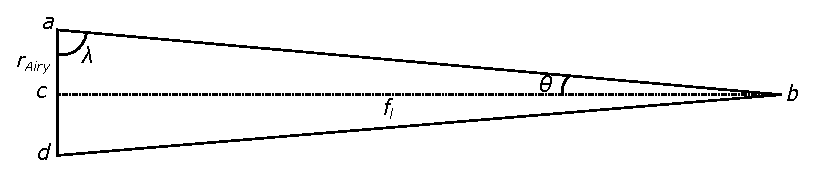
\includegraphics[]{./images/spot_size_figure.eps}
		\caption{Airy Disk Geometry}
		\label{fig:spot_geometry}
	\end{center}
\end{figure}


Here $\theta$ is the angle subtended by the radius of the Airy disk, $f_{l}$ is the focal length of the telescope and $r_{Airy}$ is the radius of the Airy disk.

The triangle abc is an right angle triangle.  From this, and from the sin rule for triangles we may say that:

\LARGE
$\frac{sin(\theta)}{r_{Airy}} = \frac{sin(\lambda)}{f_{l}}$
\large

But from the sum of internal angles in a triangle

$\lambda+\theta+90=180 \implies \lambda=90-\theta$

\LARGE
$\frac{sin(\theta)}{r_{Airy}} = \frac{sin(90-\theta)}{f_{l}}$

\LARGE
$\frac{sin(\theta)}{r_{Airy}} = \frac{cos(\theta)}{f_{l}}$

\LARGE
$r_{s}=\frac{sin(\theta)}{cos(\theta)} f_{l}$

\large
But for small values of $\theta$, $sin(\theta)\approx\theta$ and $cos(\theta)\approx 1$ thus:

\Large
\begin{equation}
\label{eqn:spot-startpoint}
r_{Airy}=\theta f_{l}
\end{equation}

\large
Substituting the value for $\theta$ derived in eqn~\ref{eqn:airy-radius} we find that:

\LARGE
$r_{Airy}=\frac{1.22\lambda f_{l}}{d} $

\Large
\begin{equation}
\label{eqn:spot-diameter}
r_{Airy}=1.22\lambda f_{r} \implies d_{Airy}=2.44\lambda f_{r}
\end{equation}

\large
Where $f_{r}$ is the focal ratio of the instrument and $d_{Airy}$ is the spot diameter.

This is actually quite a surprising result.  The spot size for an optically perfect instrument is governed by the focal ratio of the instrument.  Thus a small refractor with a focal ratio of $f_{r}$ will produce a spot size the same as a large instrument of the same focal ratio.

At first blush this appears to run counter to the notion that larger aperture instruments have finer angular resolution, but a simple diagram will illustrate this finding is in fact consistent.

\begin{figure}[htb]
	\begin{center}
		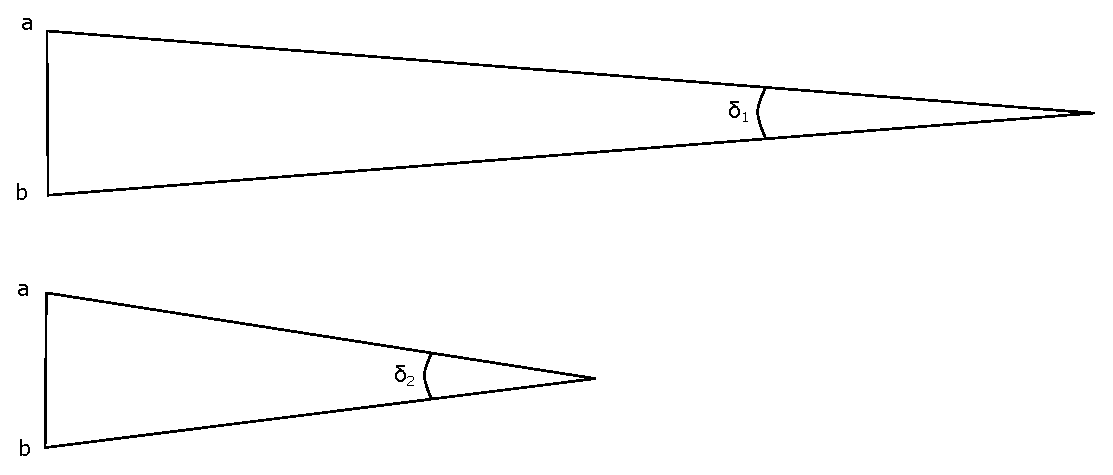
\includegraphics[scale=0.7]{./images/focal-ratio-resolution.eps}
		\caption{Spot Size and Resolution}
		\label{fig:spot_resolution}
	\end{center}
\end{figure}


Let the points {\em a} and {\em b} be the centers of 2 Airy disks that are spaced at the limit of resolution in 2 instruments of similar focal ratio but with different apertures.  Simply by observation it may be seen that $\delta_{1}$ is a smaller angle than $\delta_{2}$.  Thus the larger instrument with the longer focal length indeed has better angular resolution even though it has the same focal ratio.

\subsection{The zone of critical focus}

Now that the nature of the spot size has been established the nature of the critical focus zone (CFZ) may be examined.  

Focus in a telescope is established by moving the plane of the detector back and forth until the point of best focus is reached.  There is a point at which the spot reaches its minimum diameter, the Airy disk.  This is shown in Figure~\ref{fig:cfz}

\begin{figure}[htb]
	\begin{center}
		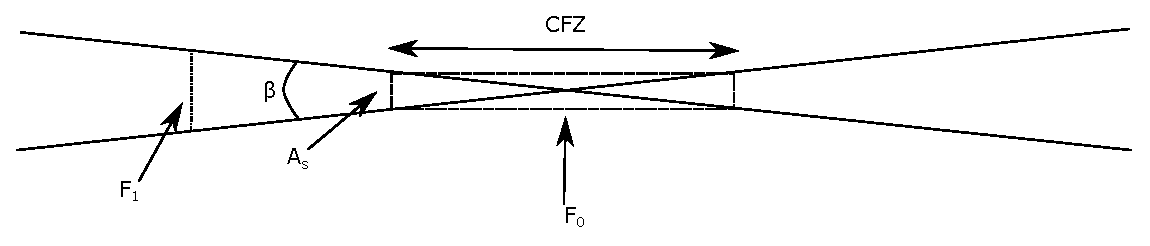
\includegraphics[scale=0.7]{./images/CFZ.eps}
		\caption{CFZ Diagram}
		\label{fig:cfz}
	\end{center}
\end{figure}

Here we see the light cone of the instrument as it extends beyond the zone of focus.  The line at $F_{1}$ indicates size of the out of focus disk on the sensor at point $F_{1}$.  

As $F_{1}$ moves towards $F_{0}$, the theoretical point of convergence of the light cone, the size of the out of focus image will reach the minimum Airy spot size indicated by $A_{s}$.  

This minimum spot size will remain unchanged on the sensor for the distance indicated by CFZ. Beyond this the spot size on the sensor will then begin to increase again.  

It should be clear then, that any change to the position of the sensor in the range given by CFZ will result in no change in the appearance of the star.  The aim then is to place the sensor within the bounds of this dead zone.

The cone angle $\beta$ is a function of the focal ratio, $f_{r}$, of the instrument.  From simple trigonometry it can be shown that $\beta$ is given by:

$\beta=2\times\arctan(\frac{1}{2f_{r}})$

To compute the physical size of the CFZ we may decompose the problem into a set of right angle triangles.

\begin{figure}[htb]
	\begin{center}
		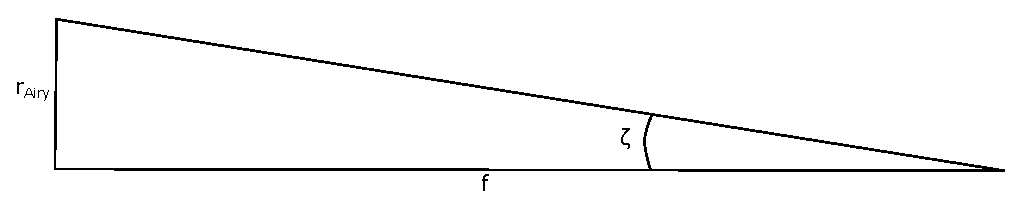
\includegraphics[]{./images/CFZ-computation.eps}
		\caption{CFZ Computation}
		\label{fig:cfz-computation}
	\end{center}
\end{figure}

$r_{Airy}$ is the Airy radius as given by equation~\ref{eqn:airy-radius}

f is half the CFZ

$\zeta$ is half the cone angle, $\zeta = arctan(\frac{1}{2f_{r}})$

Because $\zeta$ is small:

\Large
\begin{equation}
\zeta \approx \frac{1}{2f_{r}} = \frac{r_{Airy}}{f} \implies f=2r_{Airy}f_{r}
\label{eqn:physical-spot-size}
\end{equation}
\large

Substitute Eqn~\ref{eqn:airy-radius} for $r_{Airy}$:

$f=2.44\lambda f_{r}^2 \implies$

\begin{equation}
CFZ=4.88\lambda f_{r}^2
\end{equation}

Thus we may now plot the critical focus zone for yellow light for a range of focal ratios:

\begin{figure}[htb]
	\begin{center}
		\includegraphics[scale=0.7]{./images/cfz-fratio.eps}
		\caption{CFZ against Focal Ratio}
		\label{fig:cfz-plot}
	\end{center}
\end{figure}

One thing to observe is the size of the CFZ in comparison to the claimed step size of a number of commercial motorized focusing systems. It may readily be seen that the claimed resolution of many of these devices is far, far smaller than is required to achieve the optimum focus.  

This also demonstrates why depth of field of a camera lens increases as the lens is stopped down.

\newpage
\section{The effects of Seeing and Sampling}

\subsection{What seeing does to diffraction limits}
Seeing is a way of describing the turbulence in the atmosphere.  Whilst seeing effects both visual observers and astrophotographers, it is the latter that are effected most.  

The human eye can adapt rapidly to the movement of the star and can grasp moments of clarity that the imaging sensor cannot.  The human eye will form an image in a fraction of a second. An imaging sensor may take many minutes to form a usable image.

The effect for an imaging sensor is to integrate all the atmospherically induced movements with the result that the stellar image is smeared across a larger area.  In poor seeing the stars will appear larger, and the fine detail of deep space objects will be lost.


This is seen in the shape of the ideal intensity plots for stars for good seeing and bad seeing as shown in figure~\ref{fig:stellar-profiles}.

\begin{figure}[htb]
	\begin{center}
		\includegraphics[scale=0.7]{./images/stellar-profiles.eps}
		\caption{Stellar Profiles on an Imaging Sensor}
		\label{fig:stellar-profiles}
	\end{center}
\end{figure}

Over given period of time the total amount of photons received from the star does not change. The photon flux may be considered invariant. When the seeing is bad the total amount of light received is spread across a wider area than when the seeing is good. Overall, in bad seeing, the image of the star is dimmer and wider.

The width of the star is given in terms of the Full Width half Maximum value (FWHM).  The FWHM is the width of the peak at the point where the intensity is half the peak value.  The half maximum lines for good seeing and bad seeing are shown in figure~\ref{fig:stellar-profiles}.

The size of the FWHM for good seeing is considerably narrower then for bad seeing.  This will equate to stars that appear to more pin-point like and brighter in the image.

When seeing is described by astrophotographers as being 2 arcseconds or 4 arcseconds, it is the size of this FWHM value that they are referring to.
 
\subsection{Real World Critical Focus}

For the purposes of imaging at least it is very rare indeed that the performance of the optical train will be at the diffraction limit.  Rather, the performance will be limited by seeing.

How then does this effect the CFZ?  In this case,if the seeing is sufficiently bad, the smallest possible spot size will not be given by the diffraction limited value derived in equation~\ref{eqn:spot-diameter}, but instead will be limited by the FWHM value.

With reference to figure~\ref{fig:spot_geometry} we may rework the equations for the spot size but using the expression $\frac{fwhm}{2}$ for the value of $\theta$ as opposed to the expression for the angular radius of the Airy disk. Thus starting from equation~\ref{eqn:spot-startpoint}:

\Large
$r_{fwhm}=\frac{fwhm \times f_{l}}{2} $
\large

It is important to note that the value of $r_{fwhm}$ must be greater or equal to the value $r_{Airy}$.  $r_{fwhm}$ may be computed to be smaller than  $r_{Airy}$ for small values of $f_{l}$ in good seeing with low FWHM.\footnote{Strictly speaking we should in fact use half the FWHM of the Airy disk as the lower limit to be consistent. This value is slightly lower than the value of  $r_{Airy}$. For the sake of simplicity  $r_{Airy}$ is used as it is approximately equivalent for all practical purposes. }

Substituting into equation~\ref{eqn:physical-spot-size} and simplifying we get:

\begin{equation}
CFZ=2\times fwhm \times f_{l} \times f_{r}
\end{equation}

Now we see that the CFZ also depends on the focal length, $f_{l}$, of the instrument.  Previously 2 instruments of different size with similar focal ratio produced the same spot size.  

In this real world seeing limited case, the angular size of the spot that is a constant.  So a longer focal length instrument will produce a larger spot size, and a bigger CFZ.  Thus, all things being equal, in the real world a 16" RCOS at f8 will have a much larger CFZ than the otherwise equivalent 8" instrument, depending on the seeing.

A large CFZ tends to make focusing somewhat mushy , with seemingly absurdly large changes in the focus position having little or no effect on the FWHM of the stars in the image.  This tends to make critical focus harder to find, even though the dead-zone is larger.  

\subsubsection{Critical Focus Zone for various systems}

Since low cost RCOS scope have begun to become popular we will look at a hypothetical system with a focal ratio of f8 and with focal lengths from 500 mm through to 3000 mm. To simplify the mathematics the effect of the central obstruction is ignored.


\begin{figure}[htb]
	\begin{center}
		\includegraphics[scale=0.9]{./images/cfz-seeing.eps}
		\caption{CFZ for various focal lengths and seeing conditions}
		\label{fig:cfz-seeing}
	\end{center}
\end{figure}

Note that the better the seeing, the longer the CFZ will be consistent with the diffraction limit of the optics.  Also note that the longer the focal length, the sooner the CFZ departs from the diffraction limit of the optics.  

\subsection{Seeing and resolution}

Since the CFZ is directly related to the spot size of the star, we can state that longer focal length instruments need more steady skies in order to perform close to their design limits. This generally known rule-of-thumb has its basis in the physics of light.

\section{Conclusion}

Poor seeing is well known to cause issues with high resolution imaging at longer focal lengths.  It has been shown that this is directly related to the effect of the spot size of the star that is in turn governed by the seeing conditions.

Perhaps less well known is that the critical focus zone of the system is also a function of seeing.  Anyone who has struggled to find focus in less than optimal conditions need not blame their skills or  equipment.  

The laws of optics in fact require that focus will be mushy with a large critical focus zone and associated bloated stars when using longer focal length instruments in poor seeing.

In the authors case this study has caused a rethinking of what is practical under the typical Northeastern US skies.  Smaller, shorter focal length instruments are able to perform at their design limits under seeing that renders the benefits of a larger instrument marginal.  The full potential of larger instruments will not be realized.


\end{document}
